% Канонический TikZ-рисунок варианта 23. Править только здесь.
\long\def\figStereoV23{%
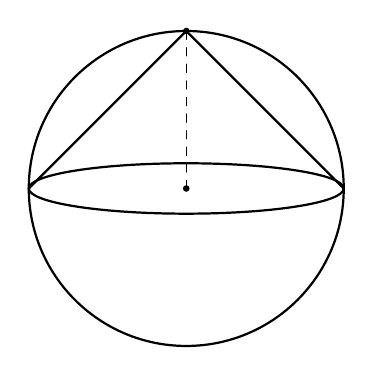
\begin{tikzpicture}[
  scale=1,
  line cap=round,
  line join=round
]
  \def\R{2}
  \def\ey{0.32}

  \coordinate (O) at (0,0);
  \coordinate (S) at (0,2);
  \coordinate (A) at (-2,0);
  \coordinate (B) at (2,0);

  % Шар
  \draw[thick] (O) circle (\R);

  % Основание конуса
  \draw[thick] (B) arc[start angle=0,end angle=180,x radius=2,y radius=\ey];
  \draw[thick] (A) arc[start angle=180,end angle=360,x radius=2,y radius=\ey];

  % Образующие конуса
  \draw[thick] (S)--(A);
  \draw[thick] (S)--(B);

  % Ось
  \draw[dashed] (S)--(O);

  \fill (S) circle (1.2pt);
  \fill (O) circle (1.2pt);
\end{tikzpicture}
}
